\chapter{MobileNetV2} \label{appendix:mbv2}
%
The structure of MobileNetV2 is illustrated in Figure \ref{fig:mbv2-struct}. According to \textcite{sandler_mobilenetv2_2018}, the structure can be described as follow: \textquote{\textit{Each line describes a sequence of 1 or more identical (modulo stride) layers, repeated n times. All layers in the same sequence have the same number c of output channels. The first layer of each sequence has a stride s and all others use stride 1. All spatial convolutions use 3 \texttimes 3 kernels. The expansion factor t is always applied to the input size}}.
\begin{figure}[H]
    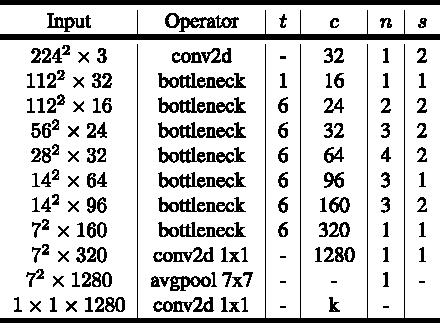
\includegraphics[width=\textwidth]{mbv2-struct.pdf}
    \caption{MobileNetV2 structure, from \cite{sandler_mobilenetv2_2018}}
    \label{fig:mbv2-struct}
\end{figure}
\newpage
